\documentclass[12pt]{article}
\usepackage{ucs}
\usepackage[utf8x]{inputenc}
\usepackage[T1]{fontenc}
\usepackage[english]{babel}
\usepackage[nottoc]{tocbibind}
\usepackage[left=2.5cm,right=2.5cm,top=2.5cm,bottom=2.5cm,]{geometry}
\usepackage{graphicx}
\usepackage{nameref}
\usepackage{hyperref}
\usepackage{sidecap}
\usepackage{wrapfig}
\usepackage[bottom,hang]{footmisc} 
\usepackage{acronym}
\usepackage{multirow}
\usepackage{color}
\usepackage{capt-of}
\usepackage{array,				%better tables
			tabularx,			%instead of tabular*             
			booktabs,			%tables for good publications
}
\usepackage{afterpage,hyperref} 
\usepackage{listings}
\lstset{
    basicstyle=\ttfamily\footnotesize,
    numbers=left,
    xleftmargin=15pt,
}


%--------------------------MAKETITLE-------------------------------%
\title{Code Similarity and Plagiarism Detection}
\date{\today}
\author{Mehmed Mustafa \\
		MatrNr: 21914377 \\
		Supervisor: Ella Albrecht} 

\begin{document}
%--------------------------BEGINNING-------------------------------%
\pagenumbering{roman} 
\maketitle
\thispagestyle{empty}
\newpage
\tableofcontents

%-----------------------SECTION START------------------------
\newpage
\pagenumbering{arabic}
\section{Introduction} \label{sec:Introduction}
In 2004 researchers reported that plagiarism is a serious threat to education and has started to increase in the past years~\cite{plagEduIncr}. Plagiarism can be described as an act of getting someone else's work and represent it as your own, of course by hiding it's source. In academia, mainly plain texts, such as reports, and source code assignments are plagiarized. A simple and good definition for source code plagiarism is given by Hage et al. "Source code plagiarism can be defined as trying to pass off (parts of) source code written by someone else as one's own (i.e., without indicating which parts are copied from which author)"~\cite{definitionSCP}. There are several actions which may lead to source-code plagiarism. Copying source code from online sources is the most obvious one. One similar action is to get source codes from the internet and convert them from one programming language to another. There are some tools which generate source codes from diagrams, and thus a student can give a diagram as an input and get source codes as an output. Yet another action is to perform source code exchange. For example, if a student is able to complete one part of the assignment, and another student is able to complete the other part, then they could exchange their parts with each other. Paying someone else to complete an assignment is also an action which may be considered by students. According to a research~\cite{schiller} there are many reasons why students plagiarize. One reason is the believe that plagiarism will go unnoticed. This believe may motivate a weak student to get the assignment of another student with, or without his/her permission, and edit it before submitting it. One other reason, why students plagiarize, is working in groups on an assignment although they are supposed to work alone. Some students may even not know that it is not acceptable. It is also possible a poorly motivated student, which is not necessarily weak, to get a code of another student and edit it just in order to decrease the amount of work needed for the completion of the assignment. According to another research~\cite{bennett} reason for plagiarism is the desire for obtaining higher grades. The reasons behind this desire of students may be the need of proving self-worth to other students, or a pathological fear of failing. Belief for better job options may also be a reason for wanting higher grades. Sometimes companies, which are looking for new employees, are doing their preliminary selection depending on the grades of freshly graduated students, thinking that higher grades mean better knowledge. Which, of course, is not always the case. Culwin et al.~\cite{plagiarismIssues} discuss why plagiarism is a problem. Firstly, students committing plagiarism and not getting punished for it, can influence other students and courage them to plagiarize. Secondly, plagiarism also affects negatively the qualification value awarded by an academic institution because students who plagiarize will not get the knowledge required for obtaining a degree. From a moral point of view, plagiarism is a form of lying, because people committing plagiarism are making others believe they are competent at something when they are not. Plagiarism can also negatively affect the creator of the plagiarized work by reducing the amount of respect they deserve or by making them lose money if this work generates an income for them. In order to reduce the impact of plagiarism on education something has to be done. One way to try to prevent plagiarism is to develop systems which will analyze and try to detect similarities among the different works. In this work, the focus is to overview plagiarism (obfuscation) methods used in academia and suggest tools for detecting them. Section 2 analyzes obfuscation methods for source code, Section 3 analyzes obfuscation methods for natural languages, Section 4 suggests plagiarism detection tools and Section 5 concludes.


\section{Obfuscation Methods for Source Code Plagiarism} \label{sec:Obfuscation Methods for Source Code Plagiarism}
 
Novak et al.~\cite{novak}, after analyzing 72 articles, which mention some kind of obfuscation methods, they have specified 16 distinct obfuscation methods, which were classified into one of the 4 categories: Lexical, Structural, Advanced Structural and Logical. The first mentioned category, Lexical, is consisted of methods, which are easiest to be detected, while the last mentioned, Logical, is consisted of methods, which are hardest to be detected. We found this classification the best in comparison to other classifications which are either not complete or it is hard for deciding in which category to put some of the obfuscation methods.


\subsection{Lexical changes} \label{sec:Lexical changes}
"Changes which could, in principle, be performed by a text editor. They do not require knowledge of the language sufficient to parse a program."~\cite{joyUndLuck} These obfuscation methods are easiest to be spotted, especially for tools which perform similarity comparisons once the code is compiled. Usually students with no to low knowledge are expected to perform lexical changes in order to try to hide their plagiarism. There are 6 obfuscation methods in this category: 

\begin{enumerate}

	\item Visual code formatting - a method by which a student would just change the amount of space, usually at the beginning of each line before the actual code, or insert new lines consistent only from whitespace characters. The opposite is also possible - removing the empty lines, which are usually set by programmers in order to improve readability;
	
	\item Comments modification - this method can include partly or fully adding, modifying or removing comments. Usually comments added by this method will be placed at places where, actually, no comment is required and the code is obvious. For example, placing "Check if grade is greater than 50" comment for this line of code "if(grade > 50)". Although this may be a clear sign which invites to have a closer look at the code, changing the comments by paraphrasing or completely deleting them has no such signs;
	
	\item Modifying program output - changing the output messages or reformatting the output shape of objects, such as tables, or changing the ~\ac{GUI} by modifying the content labels or re-positioning of labels, radio buttons and so on.  If modifying of the \ac{GUI}, however, depends on languages like HTML or CSS this modification can be classified as another obfuscation method - "reordering independent lines of code" which belongs to the "Structural changes" category;
	
	\item Identifier rename - modification of identifier names, like variable names, class names, function names, constant names and so on. Sometimes students may not change all of the identifier names, which will lead to inconsistencies in the programming style;
	
	\item Translation of program parts - this obfuscation method could be seen as a special case of the previous three methods, because translation to another language could be done for identifier names, program output and comments. For example, translating from English to another language which is native for the student performing plagiarism;
	
	\item Changing constant values - sometimes constants within a program could be changed without affecting the logic or output of the program. For instance, the , which is 3,14 could be written with higher precision - 3,1415. Although this method may look similar to identifier rename method, it may require more knowledge to be performed. In the given example, a student may also have to change the output precision to make output look similar;  
	
\end{enumerate}

\begin{figure} [ht]
    \centering
    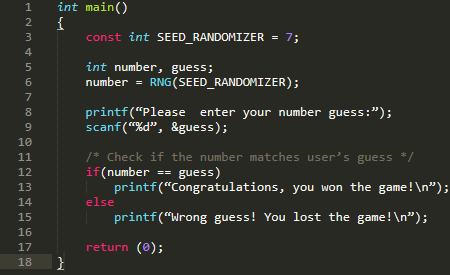
\includegraphics[width=12cm, height=7cm]{../images/sourceCodeLexical1.png}
    \caption{Original source code}
    \label{fig:sourceCodeLexical1}
\end{figure}

\begin{figure} [ht]
    \centering
    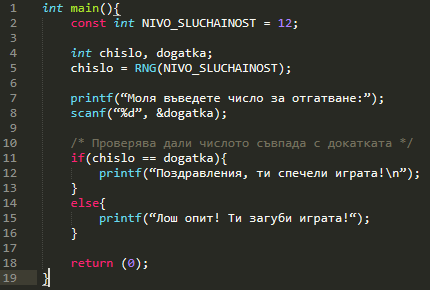
\includegraphics[width=12cm, height=7cm]{../images/sourceCodeLexical2.png}
    \caption{Plagiarized source code with lexical changes}
    \label{fig:sourceCodeLexical2}
\end{figure}

Figure~\ref{fig:sourceCodeLexical1} and Figure~\ref{fig:sourceCodeLexical2} are examples respectively for original and plagiarized source  code using lexical changes. All of the methods described above are used in the plagiarized code. Translation of program parts method covers identifier rename, modifying program output and comments modification.



\subsection{Structural changes} \label{sec:Structural changes}
"Requires the sort of knowledge of a program that would be necessary to parse it. It is highly language-dependent."~\cite{joyUndLuck} In comparison to lexical changes, which don't require any programming knowledge, structural changes require some knowledge about the connection of different lines of code. There are 4 obfuscation methods in this directory:

\begin{enumerate}

	\item Reordering independent lines of code - all kinds of line reordering which do not change the working flow of a program. Such modifications could be achieved by changing the order of variable declarations or by reordering the position of function declarations or inner classes;
	
	\item Adding redundant lines of code - could be achieved easily by adding codes to unreachable sections of the program or lines, such as "b=b;" anywhere. Fortunately, any ~\ac{IDE} would warn if there are lines of code which are unreachable or redundant, so this method is not very useful to be plagiarized with, unless the source codes are only automatically analyzed by tool which does not support the feature of the current generation development environments;
	
	\item Splitting up lines of code - the idea behind this method is to make the code seem longer than the original version. It could be performed on single line by splitting it to many lines, or splitting one class to many smaller classes, or splitting one function into many smaller functions and etc.;
	
	\item Merging lines of code - this method could be seen as the opposite of splitting. Smaller classes, functions or files could be combined into one bigger. Simplest version of this method is to combine declaration or initialization of variables in less lines;
	
\end{enumerate}

\begin{figure} [ht]
    \centering
    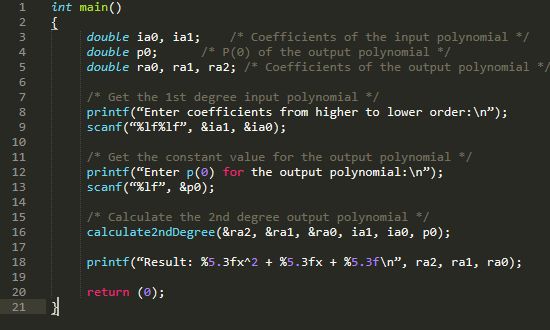
\includegraphics[width=12cm, height=7.5cm]{../images/sourceCodeStructural1.png}
    \caption{Original source code}
    \label{fig:sourceCodeStructural1}
\end{figure}

Figure~\ref{fig:sourceCodeStructural1} and Figure~\ref{fig:sourceCodeStructural2} are examples respectively for original and plagiarized source code using structural changes. For example, reordering independent lines of code and merging lines of code methods are used to transform lines 3-5 in Figure~\ref{fig:sourceCodeStructural1} to lines 3-4 in Figure~\ref{fig:sourceCodeStructural2}. Also the function call on line 16 in Figure~\ref{fig:sourceCodeStructural1} is substituted with the implementation of that function and its independent lines of code are distributed to lines 10 and 16-17 in Figure~\ref{fig:sourceCodeStructural2}. There are also lexical changes, like comments modification.

\begin{figure} [ht]
    \centering
    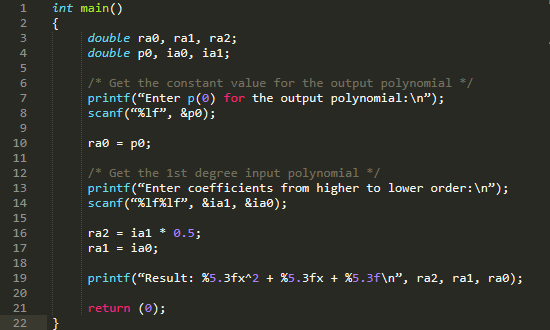
\includegraphics[width=12cm, height=7.5cm]{../images/sourceCodeStructural2.png}
    \caption{Plagiarized source code with structural changes}
    \label{fig:sourceCodeStructural2}
\end{figure}



\subsection{Advanced structural changes} \label{sec:Advanced structural changes}
"Subcategory of structural changes that require more knowledge of program possibilities and relations between equivalent statements in a specific programming language."~\cite{novak} This category is the advanced version of the previous one. Students which are able to perform these obfuscation methods have some knowledge about modifiers, control structures like if, switch, for or while and different data structures.

\begin{enumerate}

	\item Changing of statement specification - this method could be further divided in future sub methods - altering modifiers, changing data types and changing operations and operands. Altering modifiers could be performed, for example, by changing "private" variables or functions of a class to "public". Changing "float" to "double", "int" to "long int" or "arrays" to "array lists" are cases of changing data types. Modifying operands or operations in logical expressions is a bit more complicated than the previous two sub methods. For example, changing "(x == y)" to "!( x != y)" or "(x <= 5) to "(6 > x)"
	
	\item Replacing control structures with equivalents - "if" statements changed to "switch" or vice-versa is an example for this method. Other possible changes are "for" to "while" or "do...while";
	
\end{enumerate}

\begin{figure} [ht]
    \centering
    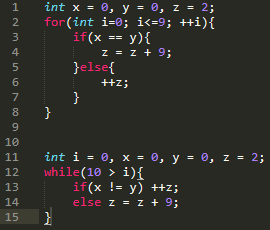
\includegraphics[width=12cm, height=7.5cm]{../images/sourceCodeAdvanced.png}
    \caption{Example of original and plagiarized code snippets}
    \label{fig:sourceCodeAdvanced}
\end{figure}

Figure~\ref{fig:sourceCodeAdvanced} shows two snippets of code, the first 8 lines are the original source code, the lines after line 10 are plagiarized using advanced structural changes. The difference between the two snippets is the exchange of looping control structure - "for" is substituted with "while" and changes in statement specifications - "x == y" in the original code is exchanged with "x != y" in the plagiarized code. Of course, the lines which are executed depending on the value of the boolean expression are also swapped to keep the functionality of the code and the output same (lines 4 and 6 are swapped in lines 13 and 14). The boolean expressions controlling the two loops are also exchanged - "i <= 9" is substituted with its equal "10 > i". These two advanced structural methods combined with lexical and structural obfuscation methods could work even better for hiding plagiarism. For example, if the variable names are changed and there are some additional comments, the two snippets of code, at first glance, will look completely different. 

\subsection{Logical changes} \label{sec:Logical changes}
"Changes that except for structural changes also change the logic (flow) of a program and require certain amount of programming skills and knowledge about the application being developed to be performed correctly."~\cite{novak} This category contains the most advanced techniques for hiding plagiarism and usually these are hard to be detected by a human or a plagiarism tools. If a student is able to use some of these methods it means that he or she has enough knowledge about programming or about the target programming language. There are 4 methods in this category:

\begin{enumerate}

	\item Simplifying the code - removing the complex or unneeded parts of the copied source code. For example, students may get an assignment in which they have to implement Dijkstra's algorithm for finding the shortest paths between nodes in a graph. There are a lot of applications using this algorithm one or another way. The students who want to plagiarize could just copy the algorithm part and leave out other details of the application;

	\item Translation of program from other programming language - converting source code written in one programming language to another. Usually code needed for an assignment or part of it could be found on the Internet, but written in another programming language and since the student performing plagiarism will also need to change some of the logic within the copied program this method is not only structural;
	
	\item Changing the logic - this method requires the most knowledge from the student's side and it is the most complicated method. Sometimes even if the student has all the programming knowledge he or she needs to complete an assignment, he or she may lack an idea how to design and implement the application or project. One other case may be when a student has completed his assignment, but created variations of his or her source code to be able to sell it to other students which are lacking skills to complete the assignment alone;
	
	\item Combining copied and original code - this obfuscation method could be either easy or very complicated to be performed depending on the level of mixing between the copied code and the original code of the student. Some logical changes may be needed for a successful mix;

\end{enumerate}


\section{Obfuscation Methods for Natural Languages}\label{sec:Obfuscation Methods for Natural Languages}
Detecting plagiarism in natural language texts is just as important as the detection of plagiarism in source codes, because students, in addition to their assignments, may have to write reports or research papers as well. However, plagiarism is not limited only to students and may be performed even by teaching assistants. There are some obfuscation methods, which are used to surpass plagiarism detection tools. Some of these methods may have already been known and the tools patched to be able to detect them.

\subsection{Substitution methods - whitespace, alphabet or words} \label{sec:Substitution methods - whitespace, alphabet or words}
We have classified the substitution methods into three subgroups, because their main and similar part is the substitution - whitespace substitutions~\cite{plainTextPlag}, latin-greek-cyrillic alphabet letters substitutions~\cite{plainTextPlag} or word(synonym) substitutions~\cite{plainTextPlag2}. These 3 methods are similar to each other. The whitespace substitution method is the action of replacing white space characters (spaces, tabs, feeds...) with another character and making the font of that character white. In the eyes of the instructor, this white font character will look like a white space character. On the other hand, the plagiarism detection tool, since there will be no white space characters, will see the whole text as a single word. Then when the tool compares it to the same text, but with white space characters, it will detect completely different content, although it is not. An easy way to detect this method is to check the words occurring inside a text and try to match them with words inside a dictionary. If there are some random white font characters placed here and there, the detection tool will fail to match them and if the matching percentage is below some level, it may be an indication that something is wrong with the submitted work. 

\begin{figure} [ht]
    \centering
    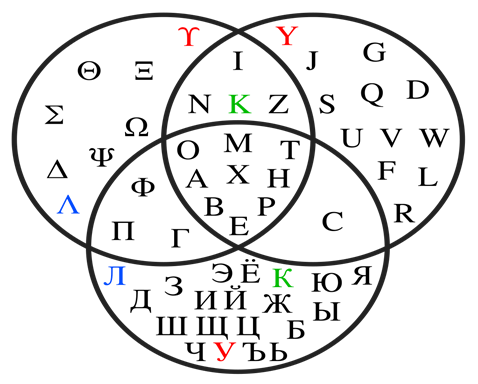
\includegraphics[width=0.50\textwidth]{../images/vennAlphabet.png}
    \caption{Similar looking letters in the Greek, Cyrillic and Latin alphabets.~\cite{vennDiagram}.}
    \label{fig:vennDiagram}
\end{figure}

The second method is similar to the first, but this time the substitution happens between letters, which have the same appearance, but different ~\ac{ASCII} code value. Figure~\ref{fig:vennDiagram} shows a Venn diagram of letters, which have the same appearance in different alphabets - Greek, Cyrillic and Latin. This obfuscation method can be countered the same way as the first one - by trying to match words to dictionary words. The last obfuscation method of this subsection is the substitution of words with their synonyms without changing the structure of sentences. This method is harder to be detected in comparison to previous two methods, because a simple word match will not help. However, the tools could still be able to label words with their synonyms as similar, if there is a synonym dictionary available for the tool. 

\subsection{Usage of "invisible" characters} \label{sec:Usage of "invisible" characters}
This method was derived by taking inspiration from the three methods above. In the Unicode character set, which is the world standard for text and can be seen as an extension of ~\ac{ASCII}, there are some special kind of characters which are invisible and are used as formatting symbols for languages like Korean and Chinese. One example is the Unicode Character with code U+3164 named Hangul Filler~\cite{hangul}. Such symbols may be used inside sentences which are plagiarized and between words of those sentences. We have tested this obfuscation method by creating 2 files with exactly the same sentence as content. Then used "invisible" characters in one of the files. Then tested on two online plagiarism detection tools. Both of them failed to detect the plagiarized sentence with exactly the same content. One of the online tools was copyleaks~\cite{copyleaks} and it gave 0\% similarity results in all of its categories: identical, minor changes and related meaning. The second tool was diffchecker~\cite{diffchecker}. Figure~\ref{fig:diffChecker} shows the results of diffchecker, which failed as well.

\begin{figure} [ht]
    \centering
    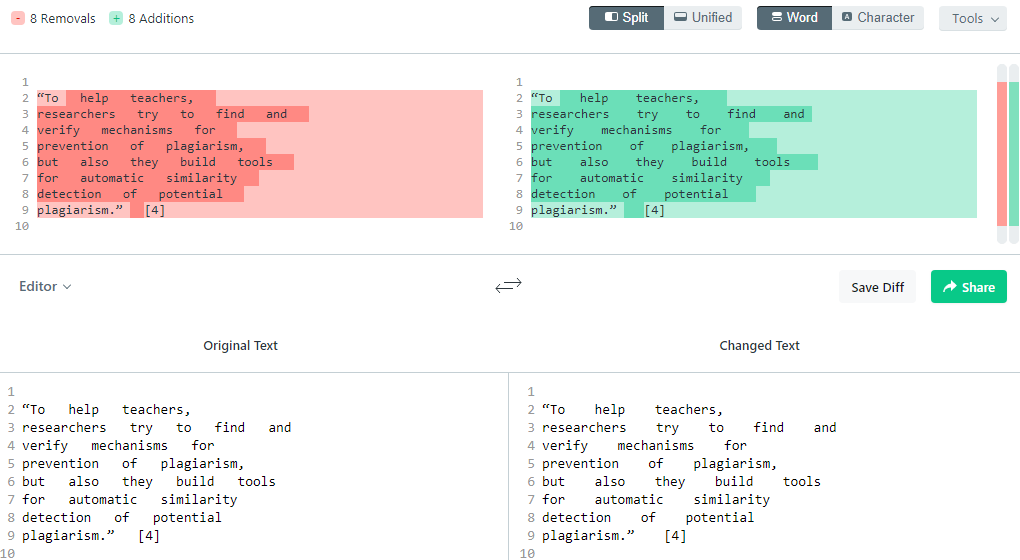
\includegraphics[width=1.0\textwidth]{../images/DiffChecker2.png}
    \caption{Online plagiarism detection tool diffchecker fails to detect plagiarized content~\cite{diffchecker}.}
    \label{fig:diffChecker}
\end{figure}

\section{Available Tools for detecting Source Code Plagiarism}\label{sec:Available Tools for detecting Source Code Plagiarism}

%WRITE HERE SOME GENERAL DETECTION %TECHNIQUES(ALGORITHMS) and which categories exist %here, for example - text based, binary based %etc...

First research papers mentioning some kind of source-code plagiarism detection are dating back to the 1970s. However, the interest in this topic has grown in the last 15 years. This statement is supported with the fact that the number of source-code detection tools has started to increase at the beginning of 21st century. Check out Figure~\ref{fig:toolsNumber}. 

\begin{figure} [ht]
    \centering
    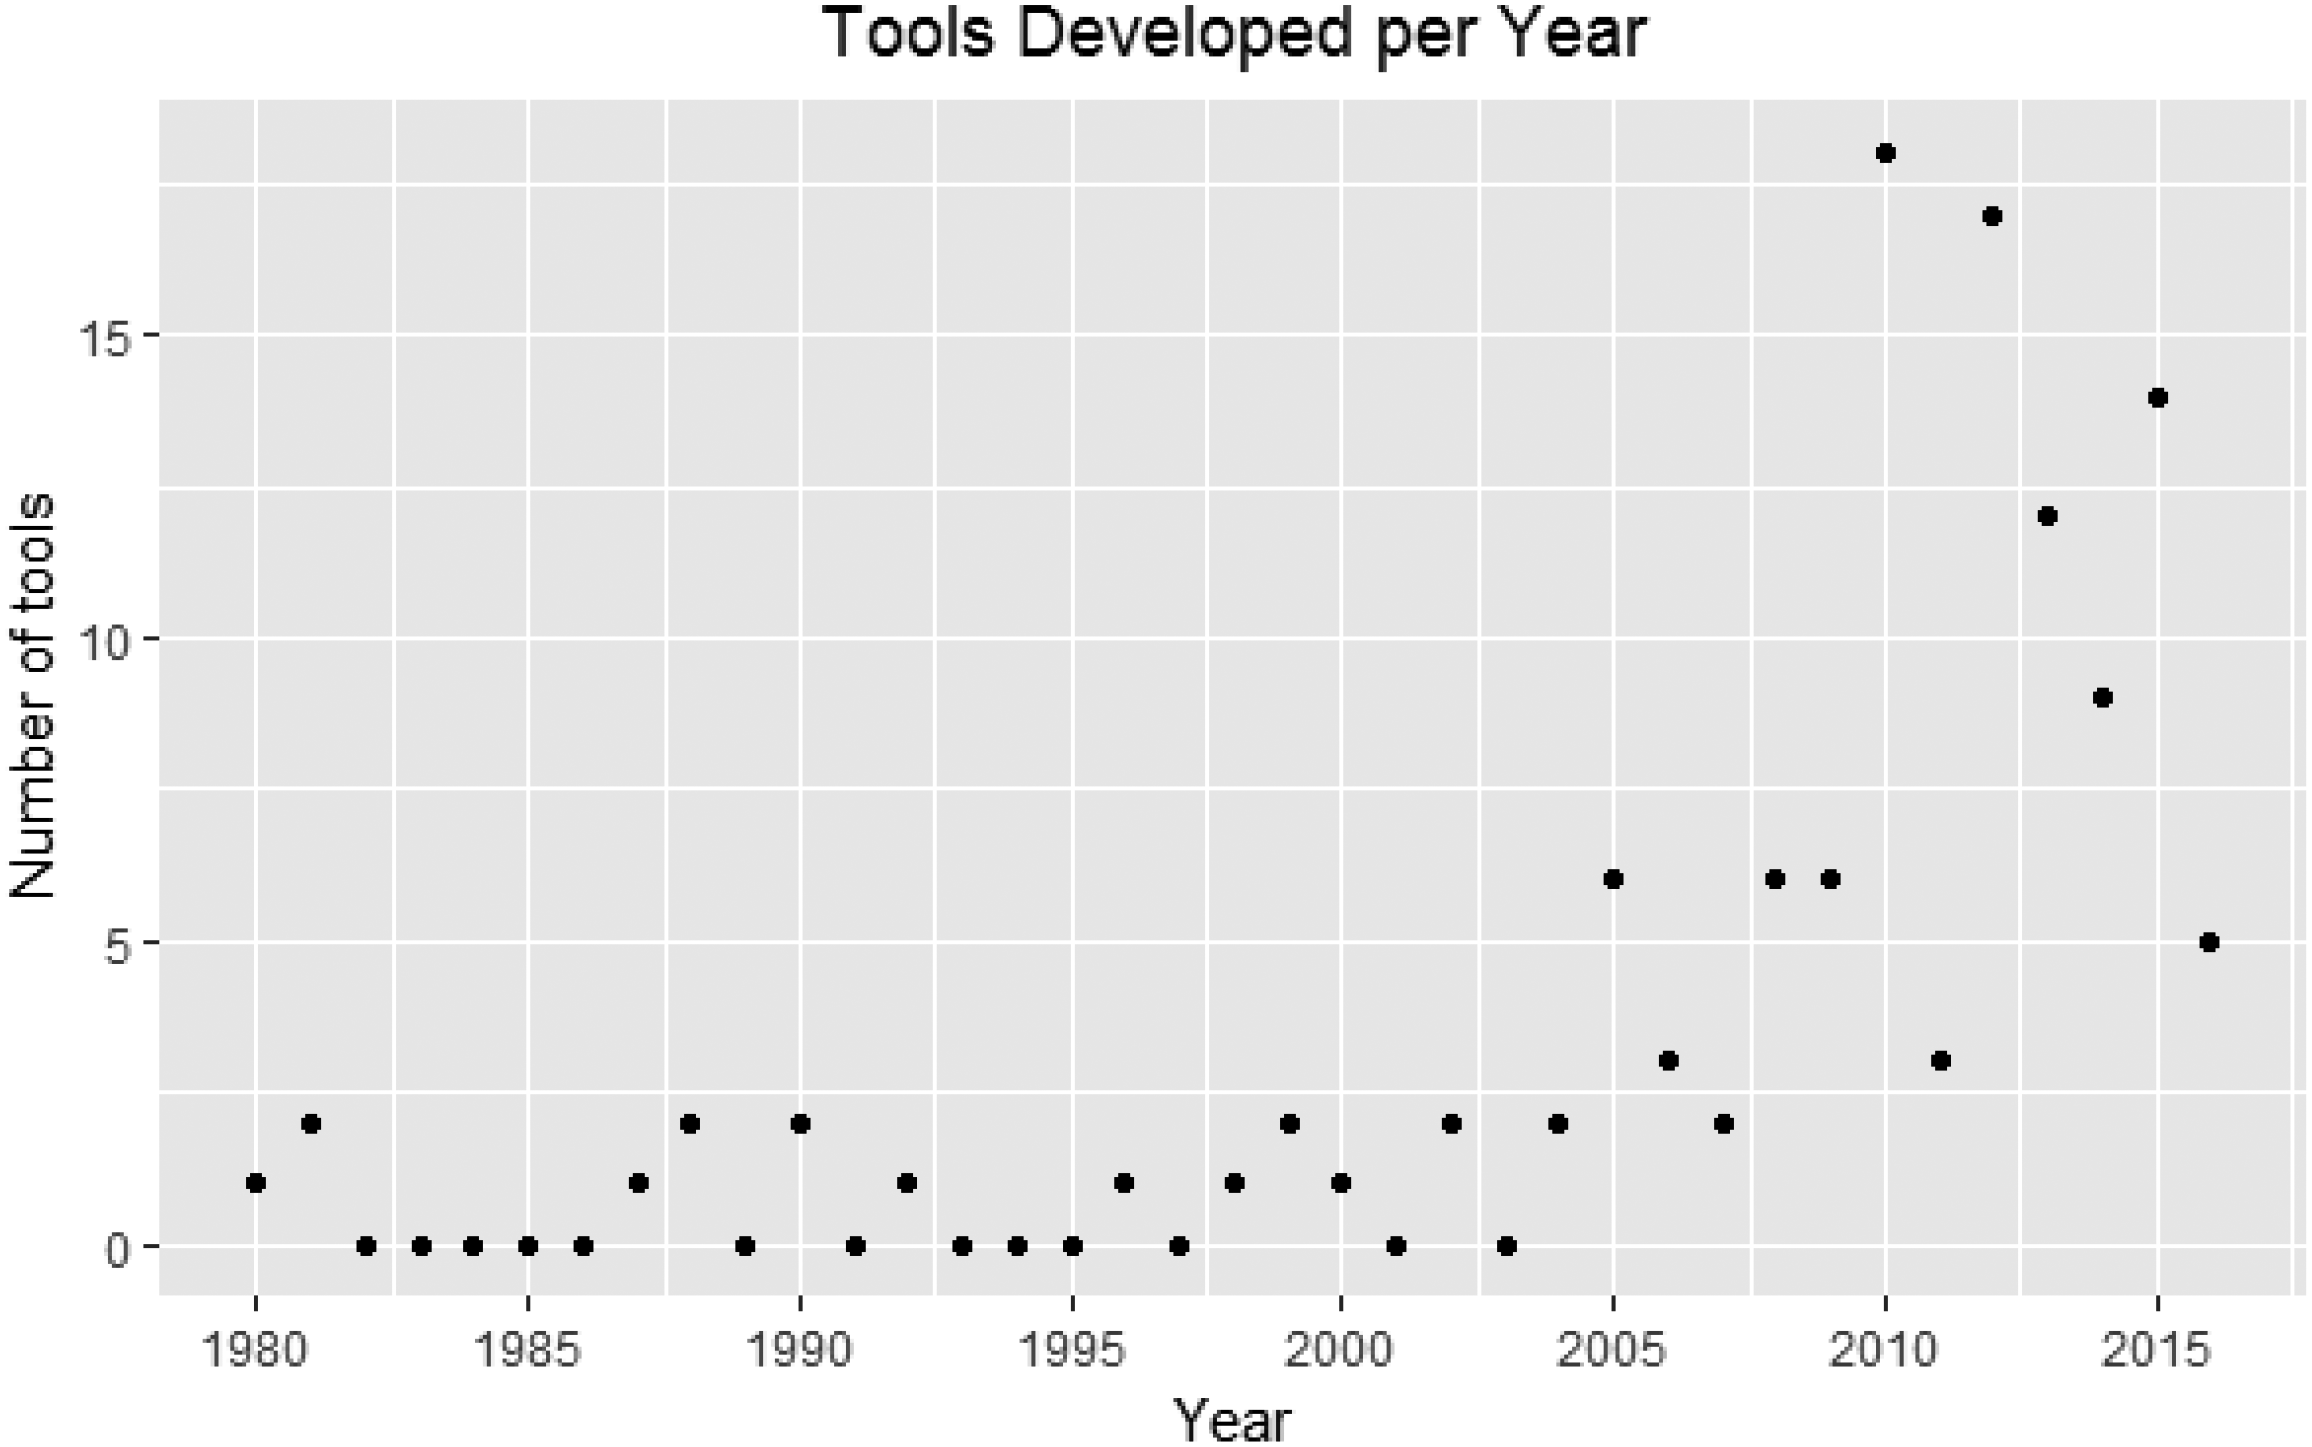
\includegraphics[width=0.65\textwidth]{../images/ToolsNumber.png}
    \caption{Number of tools developed per year.~\cite{novak}.}
    \label{fig:toolsNumber}
\end{figure}

It shows the number of tools developed per year between 1980 and 2015. If instructors use such tools for preliminary check of assignments, and then observe only works which were labeled as "highly similar", it will be easier to detect plagiarism and the motivation of students, who plagiarize or think to plagiarize, will be decreased. However, using the source-code plagiarism detection tools may not be enough for a final conclusion. Sometimes the tools may produce false results and instructors should always approach these results critically. One research paper states the following: "It is certainly safe to say that neither the detection system described in this paper nor any other detection system will find all occurrences of plagiarism. There is an inherent tradeoff between a highly discriminatory system, which overlooks some instances of cheating, and a less discriminatory one which flags many dissimilar programs."~\cite{donaldson}. Although the increased number of plagiarism detection tools in the past years, it is still hard to decide, which tools are good and for what. Novak et al.~\cite{novak} give an overview of "top-five" plagiarism detection tools. They have used two criteria to rank the tools. The first criterion is the number of mentions. The second criterion is the comparison number. A tool should have been compared to other tools at least four times to take place in the ranking. More a tool is mentioned in research papers and compared to other tools better the ranking is. 

Table~\ref{table:toolsTable} shows the "top-five" tools and gives information whether they are open source, have ~\ac{GUI} and are available offline. This ranking is not surprising, because all of the tools ranked high are free for use and most of them are open source. Hence, they are more likely to be compared and used. The selection criteria leaves out tools which are not open to the public or are developed by authors and discussed only in their research paper without comparisons to other tools, which makes the quality of the developed tool questionable. If a tool is not available for usage, although it could be the best tool ever, it has no use for researchers and instructors. Also offline availability of a tool could be a useful feature, since some universities may have privacy policy which forbids sending data of students to servers outside of the campus, and thus making tools available only online impossible for use. 

\begin{table}[ht]
\centering
\begin{tabular}{|c c c c c c|} 
 \hline
 Tool Name &  Mentions & Comparisons & Open Source & ~\acs{GUI} & Available Offline \\ [0.5ex] 
\hline
 JPlag			& 43 & 37 & YES & YES & YES\\
 MOSS			& 38 & 29 &  NO & YES & NO\\
 Sherlock-Warwick&  9 &  4 & YES & YES & YES\\
 Plaggie		&  7 &  6 & YES & YES & YES\\
 SIM-Grune 		&  6 &  4 & YES &  NO & YES\\
\hline
\end{tabular}
\caption{Top 5 plagiarism detection tools suggested by~\cite{novak}.}
\label{table:toolsTable}
\footnotetext "JPlag - https://jplag.ipd.kit.edu\\
\footnotetext "MOSS - https://theory.stanford.edu/∼aiken/moss/\\
\footnotetext "Sherlock-Warwick - http://warwick.ac.uk/iasgroup/software/sherlock\\
\footnotetext "Plaggie - https://www.cs.hut.fi/Software/Plaggie\\
\footnotetext "SIM-Grune - https://dickgrune.com/Programs/similarity\_tester\\
\end{table}



\section{Conclusion}\label{sec:Conclusion}
Most of the students are aware of the wide availability of resource on internet and they can be very creative when it comes to hiding plagiarism. Students can find solutions to their assignments and use different techniques, obfuscation methods, which may trick the instructors. Instructors should be aware enough about these techniques, so they can have some hints when trying to decide if a work is plagiarized or not. Of course, when there is a big amount of students, taking particular course, it becomes harder for the instructor to spend enough time for trying to detect plagiarism manually. Sometimes students are aware of this fact, and they feel more confident to plagiarize. If the process of detecting source-code plagiarism is automatized then students will think twice before committing source-code plagiarism. However, instructors should not depend completely on the results produced by plagiarism detection tools because sometimes they may be misleading. In order to reduce plagiarism maximally instructors could also take some additional steps. For example, they could try to avoid giving assignments that have general solutions. Moreover, they could try to give different assignments each semester, which will greatly reduce plagiarism between students from different semesters. Additionally, instructors could choose assignments that allow several interpretations. 

\newpage
%-------------------References---------------------------%
\section*{Abbreviations and Acronyms}
\addcontentsline{toc}{section}{Abbreviations and Acronyms}
\begin{acronym}[Bash]
\acro{ASCII} {\textit{American Standard Code for Information Interchange}}
\acro{IDE} {\textit{Integrated development environment}}
\acro{GUI} {\textit{Graphical User Interface}}
\acro{SCP} {\textit{Source Code Plagiarism}}

\end{acronym}

%----------------List-of-Tables--------------------%
%Comment the following lines out if you dont have tables or figures
\listoftables
\listoffigures
\bibliographystyle{plain}
\bibliography{lit}
\end{document}
